% Options for packages loaded elsewhere
\PassOptionsToPackage{unicode}{hyperref}
\PassOptionsToPackage{hyphens}{url}
\PassOptionsToPackage{dvipsnames,svgnames,x11names}{xcolor}
%
\documentclass[
]{article}

\usepackage{amsmath,amssymb}
\usepackage{lmodern}
\usepackage{iftex}
\ifPDFTeX
  \usepackage[T1]{fontenc}
  \usepackage[utf8]{inputenc}
  \usepackage{textcomp} % provide euro and other symbols
\else % if luatex or xetex
  \usepackage{unicode-math}
  \defaultfontfeatures{Scale=MatchLowercase}
  \defaultfontfeatures[\rmfamily]{Ligatures=TeX,Scale=1}
\fi
% Use upquote if available, for straight quotes in verbatim environments
\IfFileExists{upquote.sty}{\usepackage{upquote}}{}
\IfFileExists{microtype.sty}{% use microtype if available
  \usepackage[]{microtype}
  \UseMicrotypeSet[protrusion]{basicmath} % disable protrusion for tt fonts
}{}
\makeatletter
\@ifundefined{KOMAClassName}{% if non-KOMA class
  \IfFileExists{parskip.sty}{%
    \usepackage{parskip}
  }{% else
    \setlength{\parindent}{0pt}
    \setlength{\parskip}{6pt plus 2pt minus 1pt}}
}{% if KOMA class
  \KOMAoptions{parskip=half}}
\makeatother
\usepackage{xcolor}
\setlength{\emergencystretch}{3em} % prevent overfull lines
\setcounter{secnumdepth}{-\maxdimen} % remove section numbering
% Make \paragraph and \subparagraph free-standing
\ifx\paragraph\undefined\else
  \let\oldparagraph\paragraph
  \renewcommand{\paragraph}[1]{\oldparagraph{#1}\mbox{}}
\fi
\ifx\subparagraph\undefined\else
  \let\oldsubparagraph\subparagraph
  \renewcommand{\subparagraph}[1]{\oldsubparagraph{#1}\mbox{}}
\fi

\usepackage{color}
\usepackage{fancyvrb}
\newcommand{\VerbBar}{|}
\newcommand{\VERB}{\Verb[commandchars=\\\{\}]}
\DefineVerbatimEnvironment{Highlighting}{Verbatim}{commandchars=\\\{\}}
% Add ',fontsize=\small' for more characters per line
\usepackage{framed}
\definecolor{shadecolor}{RGB}{241,243,245}
\newenvironment{Shaded}{\begin{snugshade}}{\end{snugshade}}
\newcommand{\AlertTok}[1]{\textcolor[rgb]{0.68,0.00,0.00}{#1}}
\newcommand{\AnnotationTok}[1]{\textcolor[rgb]{0.37,0.37,0.37}{#1}}
\newcommand{\AttributeTok}[1]{\textcolor[rgb]{0.40,0.45,0.13}{#1}}
\newcommand{\BaseNTok}[1]{\textcolor[rgb]{0.68,0.00,0.00}{#1}}
\newcommand{\BuiltInTok}[1]{\textcolor[rgb]{0.00,0.23,0.31}{#1}}
\newcommand{\CharTok}[1]{\textcolor[rgb]{0.13,0.47,0.30}{#1}}
\newcommand{\CommentTok}[1]{\textcolor[rgb]{0.37,0.37,0.37}{#1}}
\newcommand{\CommentVarTok}[1]{\textcolor[rgb]{0.37,0.37,0.37}{\textit{#1}}}
\newcommand{\ConstantTok}[1]{\textcolor[rgb]{0.56,0.35,0.01}{#1}}
\newcommand{\ControlFlowTok}[1]{\textcolor[rgb]{0.00,0.23,0.31}{#1}}
\newcommand{\DataTypeTok}[1]{\textcolor[rgb]{0.68,0.00,0.00}{#1}}
\newcommand{\DecValTok}[1]{\textcolor[rgb]{0.68,0.00,0.00}{#1}}
\newcommand{\DocumentationTok}[1]{\textcolor[rgb]{0.37,0.37,0.37}{\textit{#1}}}
\newcommand{\ErrorTok}[1]{\textcolor[rgb]{0.68,0.00,0.00}{#1}}
\newcommand{\ExtensionTok}[1]{\textcolor[rgb]{0.00,0.23,0.31}{#1}}
\newcommand{\FloatTok}[1]{\textcolor[rgb]{0.68,0.00,0.00}{#1}}
\newcommand{\FunctionTok}[1]{\textcolor[rgb]{0.28,0.35,0.67}{#1}}
\newcommand{\ImportTok}[1]{\textcolor[rgb]{0.00,0.46,0.62}{#1}}
\newcommand{\InformationTok}[1]{\textcolor[rgb]{0.37,0.37,0.37}{#1}}
\newcommand{\KeywordTok}[1]{\textcolor[rgb]{0.00,0.23,0.31}{#1}}
\newcommand{\NormalTok}[1]{\textcolor[rgb]{0.00,0.23,0.31}{#1}}
\newcommand{\OperatorTok}[1]{\textcolor[rgb]{0.37,0.37,0.37}{#1}}
\newcommand{\OtherTok}[1]{\textcolor[rgb]{0.00,0.23,0.31}{#1}}
\newcommand{\PreprocessorTok}[1]{\textcolor[rgb]{0.68,0.00,0.00}{#1}}
\newcommand{\RegionMarkerTok}[1]{\textcolor[rgb]{0.00,0.23,0.31}{#1}}
\newcommand{\SpecialCharTok}[1]{\textcolor[rgb]{0.37,0.37,0.37}{#1}}
\newcommand{\SpecialStringTok}[1]{\textcolor[rgb]{0.13,0.47,0.30}{#1}}
\newcommand{\StringTok}[1]{\textcolor[rgb]{0.13,0.47,0.30}{#1}}
\newcommand{\VariableTok}[1]{\textcolor[rgb]{0.07,0.07,0.07}{#1}}
\newcommand{\VerbatimStringTok}[1]{\textcolor[rgb]{0.13,0.47,0.30}{#1}}
\newcommand{\WarningTok}[1]{\textcolor[rgb]{0.37,0.37,0.37}{\textit{#1}}}

\providecommand{\tightlist}{%
  \setlength{\itemsep}{0pt}\setlength{\parskip}{0pt}}\usepackage{longtable,booktabs,array}
\usepackage{calc} % for calculating minipage widths
% Correct order of tables after \paragraph or \subparagraph
\usepackage{etoolbox}
\makeatletter
\patchcmd\longtable{\par}{\if@noskipsec\mbox{}\fi\par}{}{}
\makeatother
% Allow footnotes in longtable head/foot
\IfFileExists{footnotehyper.sty}{\usepackage{footnotehyper}}{\usepackage{footnote}}
\makesavenoteenv{longtable}
\usepackage{graphicx}
\makeatletter
\def\maxwidth{\ifdim\Gin@nat@width>\linewidth\linewidth\else\Gin@nat@width\fi}
\def\maxheight{\ifdim\Gin@nat@height>\textheight\textheight\else\Gin@nat@height\fi}
\makeatother
% Scale images if necessary, so that they will not overflow the page
% margins by default, and it is still possible to overwrite the defaults
% using explicit options in \includegraphics[width, height, ...]{}
\setkeys{Gin}{width=\maxwidth,height=\maxheight,keepaspectratio}
% Set default figure placement to htbp
\makeatletter
\def\fps@figure{htbp}
\makeatother
\newlength{\cslhangindent}
\setlength{\cslhangindent}{1.5em}
\newlength{\csllabelwidth}
\setlength{\csllabelwidth}{3em}
\newlength{\cslentryspacingunit} % times entry-spacing
\setlength{\cslentryspacingunit}{\parskip}
\newenvironment{CSLReferences}[2] % #1 hanging-ident, #2 entry spacing
 {% don't indent paragraphs
  \setlength{\parindent}{0pt}
  % turn on hanging indent if param 1 is 1
  \ifodd #1
  \let\oldpar\par
  \def\par{\hangindent=\cslhangindent\oldpar}
  \fi
  % set entry spacing
  \setlength{\parskip}{#2\cslentryspacingunit}
 }%
 {}
\usepackage{calc}
\newcommand{\CSLBlock}[1]{#1\hfill\break}
\newcommand{\CSLLeftMargin}[1]{\parbox[t]{\csllabelwidth}{#1}}
\newcommand{\CSLRightInline}[1]{\parbox[t]{\linewidth - \csllabelwidth}{#1}\break}
\newcommand{\CSLIndent}[1]{\hspace{\cslhangindent}#1}

\usepackage{booktabs}
\usepackage{longtable}
\usepackage{array}
\usepackage{multirow}
\usepackage{wrapfig}
\usepackage{float}
\usepackage{colortbl}
\usepackage{pdflscape}
\usepackage{tabu}
\usepackage{threeparttable}
\usepackage{threeparttablex}
\usepackage[normalem]{ulem}
\usepackage{makecell}
\usepackage{xcolor}
\usepackage{arxiv}
\usepackage{orcidlink}
\usepackage{amsmath}
\makeatletter
\makeatother
\makeatletter
\makeatother
\makeatletter
\@ifpackageloaded{caption}{}{\usepackage{caption}}
\AtBeginDocument{%
\ifdefined\contentsname
  \renewcommand*\contentsname{Table of contents}
\else
  \newcommand\contentsname{Table of contents}
\fi
\ifdefined\listfigurename
  \renewcommand*\listfigurename{List of Figures}
\else
  \newcommand\listfigurename{List of Figures}
\fi
\ifdefined\listtablename
  \renewcommand*\listtablename{List of Tables}
\else
  \newcommand\listtablename{List of Tables}
\fi
\ifdefined\figurename
  \renewcommand*\figurename{Figure}
\else
  \newcommand\figurename{Figure}
\fi
\ifdefined\tablename
  \renewcommand*\tablename{Table}
\else
  \newcommand\tablename{Table}
\fi
}
\@ifpackageloaded{float}{}{\usepackage{float}}
\floatstyle{ruled}
\@ifundefined{c@chapter}{\newfloat{codelisting}{h}{lop}}{\newfloat{codelisting}{h}{lop}[chapter]}
\floatname{codelisting}{Listing}
\newcommand*\listoflistings{\listof{codelisting}{List of Listings}}
\makeatother
\makeatletter
\@ifpackageloaded{caption}{}{\usepackage{caption}}
\@ifpackageloaded{subcaption}{}{\usepackage{subcaption}}
\makeatother
\makeatletter
\@ifpackageloaded{tcolorbox}{}{\usepackage[many]{tcolorbox}}
\makeatother
\makeatletter
\@ifundefined{shadecolor}{\definecolor{shadecolor}{rgb}{.97, .97, .97}}
\makeatother
\makeatletter
\makeatother
\ifLuaTeX
  \usepackage{selnolig}  % disable illegal ligatures
\fi
\IfFileExists{bookmark.sty}{\usepackage{bookmark}}{\usepackage{hyperref}}
\IfFileExists{xurl.sty}{\usepackage{xurl}}{} % add URL line breaks if available
\urlstyle{same} % disable monospaced font for URLs
\hypersetup{
  pdftitle={Demo arXiv template},
  pdfauthor={Michael J Mahoney1,; Some One Else2},
  pdfkeywords={template, demo},
  colorlinks=true,
  linkcolor={blue},
  filecolor={Maroon},
  citecolor={Blue},
  urlcolor={Blue},
  pdfcreator={LaTeX via pandoc}}

\title{Demo arXiv template}
\author{Michael J Mahoney\textsuperscript{1,*} \and Some One Else\textsuperscript{2}}
\date{}

\begin{document}
\maketitle
\begin{abstract}
This document is only a demo explaining how to use the template.
\end{abstract}
\ifdefined\Shaded\renewenvironment{Shaded}{\begin{tcolorbox}[boxrule=0pt, borderline west={3pt}{0pt}{shadecolor}, interior hidden, frame hidden, sharp corners, breakable, enhanced]}{\end{tcolorbox}}\fi

\textsuperscript{1} Graduate Program in Environmental Science, State
University of New York College of Environmental Science and Forestry, 1
Forestry Drive, Syracuse, NY, 13210\\
\textsuperscript{2} Department of Sustainable Resources Management,
State University of New York College of Environmental Science and
Forestry, 1 Forestry Drive, Syracuse, NY, 13210

\textsuperscript{*} Correspondence:
\href{mailto:fake_email@fakeyfake.com}{Michael J Mahoney
\textless{}fake\_email@fakeyfake.com\textgreater{}}

\hypertarget{sec-intro}{%
\section{Introduction}\label{sec-intro}}

This is an example of how to use this template to render articles in the
standard arXiv format. Please note that this template is still in alpha
as I work out some of the mismatches between PDF output and the arXiv
style.

This quarto extension format supports PDF and HTML outputs.
\texttt{quarto-journals} is aiming at porting existing {\LaTeX} template
from journals to be used with quarto. PDF format is what require the
most work to fit the journals guideline, but Quarto offer a nice
rendering for HTML output too. This template only uses basic HTML format
without any customization for now.

\hypertarget{demo-of-some-features-found-in-this-demo-journal-template}{%
\section{Demo of some features found in this demo journal
template}\label{demo-of-some-features-found-in-this-demo-journal-template}}

\hypertarget{sec-shortcode}{%
\subsection{Shortcode demo}\label{sec-shortcode}}

PDF are rendered using {\LaTeX} but it is best if one can use a Markdown
syntax for cross format support.

\hypertarget{sec-chunks}{%
\subsection{Code chunk}\label{sec-chunks}}

This format hide chunks by default:

\begin{figure}

{\centering 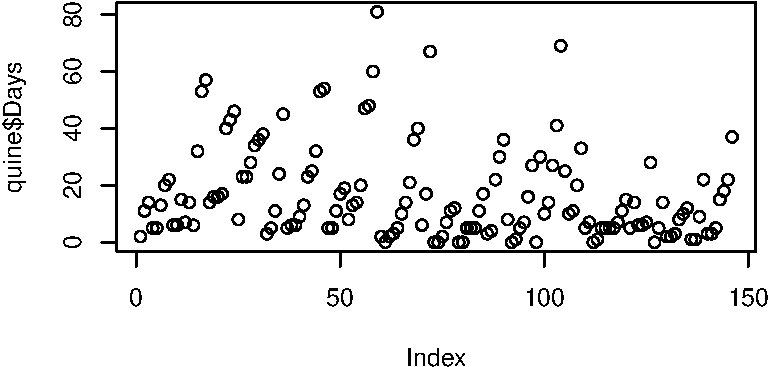
\includegraphics{template_files/figure-pdf/unnamed-chunk-1-1.pdf}

}

\caption{A figure.}

\end{figure}

But you can set \texttt{echo} option to \texttt{true} locally in the
chunk:

\begin{Shaded}
\begin{Highlighting}[]
\CommentTok{\# install.packages("broom")}
\CommentTok{\# install.packages("kableExtra")}
\NormalTok{m\_pois }\OtherTok{\textless{}{-}} \FunctionTok{glm}\NormalTok{(Days }\SpecialCharTok{\textasciitilde{}}\NormalTok{ (Eth }\SpecialCharTok{+}\NormalTok{ Sex }\SpecialCharTok{+}\NormalTok{ Age }\SpecialCharTok{+}\NormalTok{ Lrn)}\SpecialCharTok{\^{}}\DecValTok{2}\NormalTok{, }\AttributeTok{data =}\NormalTok{ quine, }\AttributeTok{family =}\NormalTok{ poisson)}
\NormalTok{kableExtra}\SpecialCharTok{::}\FunctionTok{kbl}\NormalTok{(broom}\SpecialCharTok{::}\FunctionTok{tidy}\NormalTok{(m\_pois))}
\end{Highlighting}
\end{Shaded}

\begin{table}
\caption{A table.}\tabularnewline

\centering
\begin{tabular}[t]{l|r|r|r|r}
\hline
term & estimate & std.error & statistic & p.value\\
\hline
(Intercept) & 2.9324591 & 0.0982638 & 29.8427305 & 0.0000000\\
\hline
EthN & -0.1739938 & 0.1213351 & -1.4339937 & 0.1515741\\
\hline
SexM & -0.7145197 & 0.1222943 & -5.8426235 & 0.0000000\\
\hline
AgeF1 & -0.0426993 & 0.1269111 & -0.3364507 & 0.7365310\\
\hline
AgeF2 & -0.0863239 & 0.1616403 & -0.5340495 & 0.5933073\\
\hline
AgeF3 & -0.1528978 & 0.1189753 & -1.2851227 & 0.1987494\\
\hline
LrnSL & 0.2160818 & 0.1455811 & 1.4842716 & 0.1377369\\
\hline
EthN:SexM & 0.4390243 & 0.0920790 & 4.7679077 & 0.0000019\\
\hline
EthN:AgeF1 & -0.9288934 & 0.1465738 & -6.3373786 & 0.0000000\\
\hline
EthN:AgeF2 & -1.3339773 & 0.1350383 & -9.8785113 & 0.0000000\\
\hline
EthN:AgeF3 & -0.1124246 & 0.1347842 & -0.8341080 & 0.4042202\\
\hline
EthN:LrnSL & 0.2641524 & 0.1137843 & 2.3215200 & 0.0202588\\
\hline
SexM:AgeF1 & -0.0556536 & 0.1630311 & -0.3413682 & 0.7328264\\
\hline
SexM:AgeF2 & 1.0994244 & 0.1528125 & 7.1945973 & 0.0000000\\
\hline
SexM:AgeF3 & 1.1594892 & 0.1385899 & 8.3663319 & 0.0000000\\
\hline
SexM:LrnSL & 0.0414270 & 0.1371756 & 0.3019998 & 0.7626522\\
\hline
AgeF1:LrnSL & -0.1301879 & 0.1568800 & -0.8298561 & 0.4066201\\
\hline
AgeF2:LrnSL & 0.3734020 & 0.1456293 & 2.5640585 & 0.0103456\\
\hline
AgeF3:LrnSL & NA & NA & NA & NA\\
\hline
\end{tabular}
\end{table}

\hypertarget{using-references}{%
\subsection*{Using references}\label{using-references}}
\addcontentsline{toc}{subsection}{Using references}

I did not read this book (Cameron and Trivedi 2013) but it must be
interesting

\newpage{}

\hypertarget{references}{%
\section*{References}\label{references}}
\addcontentsline{toc}{section}{References}

\hypertarget{refs}{}
\begin{CSLReferences}{1}{0}
\leavevmode\vadjust pre{\hypertarget{ref-CameronTrivedi2013}{}}%
Cameron, A. Colin, and Pravin K. Trivedi. 2013. \emph{Regression
Analysis of Count Data}. 2nd ed. Cambridge: Cambridge University Press.

\end{CSLReferences}



\end{document}
